\section{Objective}

As we discussed in the previous chapter, a internal benchmarking framework suffers from several limitations.
Not enough precision and large overhead are issues that could be solved by using an external benchmarking framework.
Such framework would be based on an external device linked to our benchmarked board.
The figure \ref{fig:external-bench-layers} represents the layers of this model and it can be divided in three parts.

\begin{figure}[!ht]
  \centering
  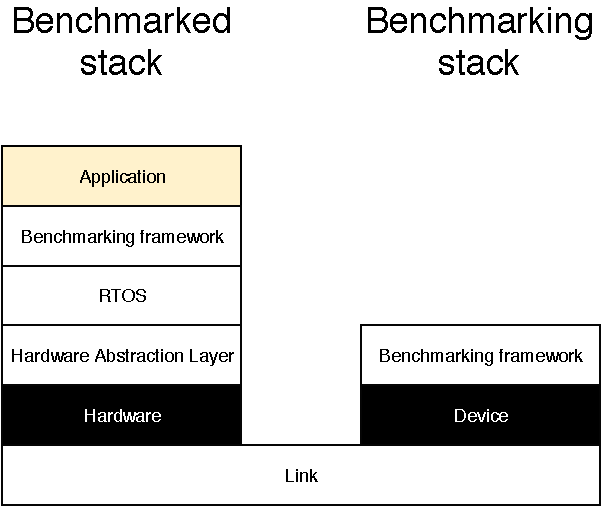
\includegraphics[scale=1]{assets/external-bench-layers.pdf}
  \caption{\label{fig:external-bench-layers}External benchmarking framework layers}
\end{figure}

\paragraph{Benchmarking stack}
The stack on the right contains our framework with the device on which the framework will run.

\paragraph{Benchmarked stack}
The stack on the left contains the application, the RTOS, the HAL, the hardware and a layer for the benchmarking framework.
This last layer between the application and the RTOS ones is kept in the benchmarked stack to communicate to our external benchmarking framework.

\paragraph{Link layer}
Finally, a link layer is represented below the two stacks.
This layer is used to communicate between the benchmarked RTOS and the benchmarking framework.

\subsection{Use case}
Ideally, our use case for this external framework is the same as presented in the previous chapter with the internal framework.

A developer should be able to run this framework with the minimum amount of configuration.
By using the framework, the developer will be able to measure the performances of its application in order to optimise it and, also, try other RTOS and other boards.